% Created by tikzDevice version 0.12 on 2019-07-24 15:39:09
% !TEX encoding = UTF-8 Unicode
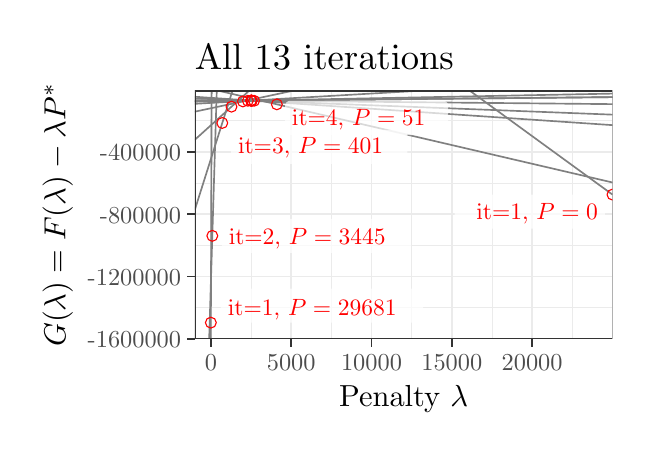
\begin{tikzpicture}[x=1pt,y=1pt]
\definecolor{fillColor}{RGB}{255,255,255}
\path[use as bounding box,fill=fillColor,fill opacity=0.00] (0,0) rectangle (216.81,144.54);
\begin{scope}
\path[clip] (  0.00,  0.00) rectangle (216.81,144.54);
\definecolor{drawColor}{RGB}{255,255,255}
\definecolor{fillColor}{RGB}{255,255,255}

\path[draw=drawColor,line width= 0.6pt,line join=round,line cap=round,fill=fillColor] (  0.00,  0.00) rectangle (216.81,144.54);
\end{scope}
\begin{scope}
\path[clip] ( 60.39, 32.08) rectangle (211.31,121.66);
\definecolor{fillColor}{RGB}{255,255,255}

\path[fill=fillColor] ( 60.39, 32.08) rectangle (211.31,121.66);
\definecolor{drawColor}{gray}{0.92}

\path[draw=drawColor,line width= 0.3pt,line join=round] ( 60.39, 43.35) --
	(211.31, 43.35);

\path[draw=drawColor,line width= 0.3pt,line join=round] ( 60.39, 65.89) --
	(211.31, 65.89);

\path[draw=drawColor,line width= 0.3pt,line join=round] ( 60.39, 88.42) --
	(211.31, 88.42);

\path[draw=drawColor,line width= 0.3pt,line join=round] ( 60.39,110.96) --
	(211.31,110.96);

\path[draw=drawColor,line width= 0.3pt,line join=round] ( 80.71, 32.08) --
	( 80.71,121.66);

\path[draw=drawColor,line width= 0.3pt,line join=round] (109.73, 32.08) --
	(109.73,121.66);

\path[draw=drawColor,line width= 0.3pt,line join=round] (138.75, 32.08) --
	(138.75,121.66);

\path[draw=drawColor,line width= 0.3pt,line join=round] (167.78, 32.08) --
	(167.78,121.66);

\path[draw=drawColor,line width= 0.3pt,line join=round] (196.80, 32.08) --
	(196.80,121.66);

\path[draw=drawColor,line width= 0.3pt,line join=round] (211.31, 32.08) --
	(211.31,121.66);

\path[draw=drawColor,line width= 0.6pt,line join=round] ( 60.39, 32.08) --
	(211.31, 32.08);

\path[draw=drawColor,line width= 0.6pt,line join=round] ( 60.39, 54.62) --
	(211.31, 54.62);

\path[draw=drawColor,line width= 0.6pt,line join=round] ( 60.39, 77.15) --
	(211.31, 77.15);

\path[draw=drawColor,line width= 0.6pt,line join=round] ( 60.39, 99.69) --
	(211.31, 99.69);

\path[draw=drawColor,line width= 0.6pt,line join=round] ( 66.19, 32.08) --
	( 66.19,121.66);

\path[draw=drawColor,line width= 0.6pt,line join=round] ( 95.22, 32.08) --
	( 95.22,121.66);

\path[draw=drawColor,line width= 0.6pt,line join=round] (124.24, 32.08) --
	(124.24,121.66);

\path[draw=drawColor,line width= 0.6pt,line join=round] (153.26, 32.08) --
	(153.26,121.66);

\path[draw=drawColor,line width= 0.6pt,line join=round] (182.29, 32.08) --
	(182.29,121.66);
\definecolor{drawColor}{gray}{0.50}

\path[draw=drawColor,line width= 0.6pt,line join=round] ( 66.06,  0.00) -- ( 66.57,144.54);

\path[draw=drawColor,line width= 0.6pt,line join=round] (128.46,144.54) -- (211.31, 84.23);

\path[draw=drawColor,line width= 0.6pt,line join=round] ( 64.60,  0.00) -- ( 69.02,144.54);

\path[draw=drawColor,line width= 0.6pt,line join=round] ( 60.39, 78.69) -- ( 81.20,144.54);

\path[draw=drawColor,line width= 0.6pt,line join=round] ( 60.39,123.75) -- (211.31, 88.60);

\path[draw=drawColor,line width= 0.6pt,line join=round] ( 60.39,104.02) -- (105.28,144.54);

\path[draw=drawColor,line width= 0.6pt,line join=round] ( 60.39,114.18) -- (202.57,144.54);

\path[draw=drawColor,line width= 0.6pt,line join=round] ( 60.39,119.58) -- (211.31,109.32);

\path[draw=drawColor,line width= 0.6pt,line join=round] ( 60.39,117.02) -- (211.31,125.80);

\path[draw=drawColor,line width= 0.6pt,line join=round] ( 60.39,117.78) -- (211.31,120.71);

\path[draw=drawColor,line width= 0.6pt,line join=round] ( 60.39,118.97) -- (211.31,113.11);

\path[draw=drawColor,line width= 0.6pt,line join=round] ( 60.39,118.37) -- (211.31,116.91);

\path[draw=drawColor,line width= 0.6pt,line join=round] ( 60.39,117.98) -- (211.31,119.44);

\path[draw=drawColor,line width= 0.6pt,line join=round] ( 60.39,117.98) -- (211.31,119.44);
\definecolor{fillColor}{RGB}{255,255,255}

\path[fill=fillColor,fill opacity=0.70] ( 71.65, 37.95) --
	(141.04, 37.95) --
	(140.97, 37.95) --
	(141.26, 37.96) --
	(141.55, 38.02) --
	(141.82, 38.12) --
	(142.07, 38.27) --
	(142.29, 38.45) --
	(142.49, 38.67) --
	(142.64, 38.92) --
	(142.76, 39.18) --
	(142.83, 39.47) --
	(142.85, 39.76) --
	(142.85, 39.76) --
	(142.85, 48.47) --
	(142.85, 48.47) --
	(142.83, 48.76) --
	(142.76, 49.05) --
	(142.64, 49.31) --
	(142.49, 49.56) --
	(142.29, 49.78) --
	(142.07, 49.96) --
	(141.82, 50.11) --
	(141.55, 50.21) --
	(141.26, 50.27) --
	(141.04, 50.28) --
	( 71.65, 50.28) --
	( 71.87, 50.27) --
	( 71.58, 50.28) --
	( 71.29, 50.24) --
	( 71.01, 50.16) --
	( 70.75, 50.04) --
	( 70.51, 49.87) --
	( 70.30, 49.67) --
	( 70.12, 49.44) --
	( 69.99, 49.18) --
	( 69.90, 48.91) --
	( 69.85, 48.62) --
	( 69.84, 48.47) --
	( 69.84, 39.76) --
	( 69.85, 39.90) --
	( 69.85, 39.61) --
	( 69.90, 39.32) --
	( 69.99, 39.05) --
	( 70.12, 38.79) --
	( 70.30, 38.56) --
	( 70.51, 38.36) --
	( 70.75, 38.19) --
	( 71.01, 38.07) --
	( 71.29, 37.99) --
	( 71.58, 37.95) --
	cycle;
\end{scope}
\begin{scope}
\path[clip] ( 60.39, 32.08) rectangle (211.31,121.66);
\definecolor{drawColor}{RGB}{255,0,0}

\node[text=drawColor,anchor=base west,inner sep=0pt, outer sep=0pt, scale=  0.85] at ( 72.37, 40.52) {it=1, $P=29681$};
\definecolor{fillColor}{RGB}{255,255,255}

\path[fill=fillColor,fill opacity=0.70] (156.09, 71.90) --
	(206.79, 71.90) --
	(206.71, 71.90) --
	(207.01, 71.91) --
	(207.29, 71.97) --
	(207.56, 72.07) --
	(207.81, 72.22) --
	(208.04, 72.40) --
	(208.23, 72.62) --
	(208.39, 72.87) --
	(208.50, 73.13) --
	(208.57, 73.42) --
	(208.59, 73.71) --
	(208.59, 73.71) --
	(208.59, 82.42) --
	(208.59, 82.42) --
	(208.57, 82.71) --
	(208.50, 83.00) --
	(208.39, 83.26) --
	(208.23, 83.51) --
	(208.04, 83.73) --
	(207.81, 83.91) --
	(207.56, 84.06) --
	(207.29, 84.16) --
	(207.01, 84.22) --
	(206.79, 84.23) --
	(156.09, 84.23) --
	(156.31, 84.22) --
	(156.02, 84.23) --
	(155.73, 84.19) --
	(155.45, 84.11) --
	(155.19, 83.99) --
	(154.95, 83.82) --
	(154.74, 83.62) --
	(154.56, 83.39) --
	(154.43, 83.13) --
	(154.34, 82.86) --
	(154.29, 82.57) --
	(154.28, 82.42) --
	(154.28, 73.71) --
	(154.29, 73.85) --
	(154.29, 73.56) --
	(154.34, 73.27) --
	(154.43, 73.00) --
	(154.56, 72.74) --
	(154.74, 72.51) --
	(154.95, 72.31) --
	(155.19, 72.14) --
	(155.45, 72.02) --
	(155.73, 71.94) --
	(156.02, 71.90) --
	cycle;
\end{scope}
\begin{scope}
\path[clip] ( 60.39, 32.08) rectangle (211.31,121.66);
\definecolor{drawColor}{RGB}{255,0,0}

\node[text=drawColor,anchor=base east,inner sep=0pt, outer sep=0pt, scale=  0.85] at (206.07, 75.35) {it=1, $P=0$};
\definecolor{fillColor}{RGB}{255,255,255}

\path[fill=fillColor,fill opacity=0.70] ( 71.94, 63.16) --
	(136.66, 63.16) --
	(136.59, 63.16) --
	(136.88, 63.17) --
	(137.17, 63.23) --
	(137.44, 63.33) --
	(137.69, 63.47) --
	(137.91, 63.66) --
	(138.11, 63.88) --
	(138.26, 64.12) --
	(138.38, 64.39) --
	(138.45, 64.67) --
	(138.47, 64.96) --
	(138.47, 64.96) --
	(138.47, 73.68) --
	(138.47, 73.68) --
	(138.45, 73.97) --
	(138.38, 74.25) --
	(138.26, 74.52) --
	(138.11, 74.77) --
	(137.91, 74.98) --
	(137.69, 75.17) --
	(137.44, 75.31) --
	(137.17, 75.42) --
	(136.88, 75.47) --
	(136.66, 75.49) --
	( 71.94, 75.49) --
	( 72.16, 75.47) --
	( 71.87, 75.49) --
	( 71.58, 75.45) --
	( 71.30, 75.37) --
	( 71.04, 75.24) --
	( 70.80, 75.08) --
	( 70.59, 74.88) --
	( 70.42, 74.65) --
	( 70.28, 74.39) --
	( 70.19, 74.11) --
	( 70.14, 73.83) --
	( 70.14, 73.68) --
	( 70.14, 64.96) --
	( 70.14, 65.11) --
	( 70.14, 64.82) --
	( 70.19, 64.53) --
	( 70.28, 64.25) --
	( 70.42, 64.00) --
	( 70.59, 63.76) --
	( 70.80, 63.56) --
	( 71.04, 63.40) --
	( 71.30, 63.27) --
	( 71.58, 63.19) --
	( 71.87, 63.16) --
	cycle;
\end{scope}
\begin{scope}
\path[clip] ( 60.39, 32.08) rectangle (211.31,121.66);
\definecolor{drawColor}{RGB}{255,0,0}

\node[text=drawColor,anchor=base west,inner sep=0pt, outer sep=0pt, scale=  0.85] at ( 72.66, 66.17) {it=2, $P=3445$};
\definecolor{fillColor}{RGB}{255,255,255}

\path[fill=fillColor,fill opacity=0.70] ( 75.30, 95.30) --
	(135.35, 95.30) --
	(135.28, 95.30) --
	(135.57, 95.31) --
	(135.85, 95.37) --
	(136.12, 95.48) --
	(136.38, 95.62) --
	(136.60, 95.81) --
	(136.79, 96.02) --
	(136.95, 96.27) --
	(137.06, 96.54) --
	(137.13, 96.82) --
	(137.16, 97.11) --
	(137.16, 97.11) --
	(137.16,105.83) --
	(137.16,105.83) --
	(137.13,106.12) --
	(137.06,106.40) --
	(136.95,106.67) --
	(136.79,106.91) --
	(136.60,107.13) --
	(136.38,107.31) --
	(136.12,107.46) --
	(135.85,107.56) --
	(135.57,107.62) --
	(135.35,107.63) --
	( 75.30,107.63) --
	( 75.52,107.62) --
	( 75.23,107.63) --
	( 74.94,107.60) --
	( 74.66,107.52) --
	( 74.40,107.39) --
	( 74.16,107.23) --
	( 73.95,107.02) --
	( 73.78,106.79) --
	( 73.64,106.53) --
	( 73.55,106.26) --
	( 73.50,105.97) --
	( 73.50,105.83) --
	( 73.50, 97.11) --
	( 73.50, 97.25) --
	( 73.50, 96.96) --
	( 73.55, 96.68) --
	( 73.64, 96.40) --
	( 73.78, 96.14) --
	( 73.95, 95.91) --
	( 74.16, 95.71) --
	( 74.40, 95.54) --
	( 74.66, 95.42) --
	( 74.94, 95.34) --
	( 75.23, 95.30) --
	cycle;
\end{scope}
\begin{scope}
\path[clip] ( 60.39, 32.08) rectangle (211.31,121.66);
\definecolor{drawColor}{RGB}{255,0,0}

\node[text=drawColor,anchor=base west,inner sep=0pt, outer sep=0pt, scale=  0.85] at ( 76.02, 98.93) {it=3, $P=401$};
\definecolor{fillColor}{RGB}{255,255,255}

\path[fill=fillColor,fill opacity=0.70] ( 94.79,105.74) --
	(150.17,105.74) --
	(150.09,105.75) --
	(150.38,105.76) --
	(150.67,105.82) --
	(150.94,105.92) --
	(151.19,106.06) --
	(151.42,106.25) --
	(151.61,106.47) --
	(151.77,106.71) --
	(151.88,106.98) --
	(151.95,107.26) --
	(151.97,107.55) --
	(151.97,107.55) --
	(151.97,116.27) --
	(151.97,116.27) --
	(151.95,116.56) --
	(151.88,116.84) --
	(151.77,117.11) --
	(151.61,117.36) --
	(151.42,117.57) --
	(151.19,117.76) --
	(150.94,117.90) --
	(150.67,118.01) --
	(150.38,118.06) --
	(150.17,118.08) --
	( 94.79,118.08) --
	( 95.01,118.06) --
	( 94.72,118.08) --
	( 94.43,118.04) --
	( 94.15,117.96) --
	( 93.89,117.83) --
	( 93.65,117.67) --
	( 93.44,117.47) --
	( 93.27,117.24) --
	( 93.13,116.98) --
	( 93.04,116.70) --
	( 92.99,116.42) --
	( 92.99,116.27) --
	( 92.99,107.55) --
	( 92.99,107.70) --
	( 92.99,107.41) --
	( 93.04,107.12) --
	( 93.13,106.84) --
	( 93.27,106.59) --
	( 93.44,106.35) --
	( 93.65,106.15) --
	( 93.89,105.99) --
	( 94.15,105.86) --
	( 94.43,105.78) --
	( 94.72,105.75) --
	cycle;
\end{scope}
\begin{scope}
\path[clip] ( 60.39, 32.08) rectangle (211.31,121.66);
\definecolor{drawColor}{RGB}{255,0,0}

\node[text=drawColor,anchor=base west,inner sep=0pt, outer sep=0pt, scale=  0.85] at ( 95.51,109.11) {it=4, $P=51$};

\path[draw=drawColor,line width= 0.4pt,line join=round,line cap=round] ( 66.19, 37.95) circle (  1.96);

\path[draw=drawColor,line width= 0.4pt,line join=round,line cap=round] (211.31, 84.23) circle (  1.96);

\path[draw=drawColor,line width= 0.4pt,line join=round,line cap=round] ( 66.72, 69.32) circle (  1.96);

\path[draw=drawColor,line width= 0.4pt,line join=round,line cap=round] ( 70.32,110.10) circle (  1.96);

\path[draw=drawColor,line width= 0.4pt,line join=round,line cap=round] ( 90.04,116.84) circle (  1.96);

\path[draw=drawColor,line width= 0.4pt,line join=round,line cap=round] ( 73.65,115.99) circle (  1.96);

\path[draw=drawColor,line width= 0.4pt,line join=round,line cap=round] ( 77.77,117.89) circle (  1.96);

\path[draw=drawColor,line width= 0.4pt,line join=round,line cap=round] ( 81.82,118.12) circle (  1.96);

\path[draw=drawColor,line width= 0.4pt,line join=round,line cap=round] ( 79.56,118.13) circle (  1.96);

\path[draw=drawColor,line width= 0.4pt,line join=round,line cap=round] ( 80.70,118.17) circle (  1.96);

\path[draw=drawColor,line width= 0.4pt,line join=round,line cap=round] ( 80.99,118.17) circle (  1.96);

\path[draw=drawColor,line width= 0.4pt,line join=round,line cap=round] ( 80.87,118.17) circle (  1.96);

\path[draw=drawColor,line width= 0.4pt,line join=round,line cap=round] ( 80.82,118.17) circle (  1.96);

\path[draw=drawColor,line width= 0.4pt,line join=round,line cap=round] ( 80.83,118.17) circle (  1.96);
\definecolor{drawColor}{gray}{0.20}

\path[draw=drawColor,line width= 0.6pt,line join=round,line cap=round] ( 60.39, 32.08) rectangle (211.31,121.66);
\end{scope}
\begin{scope}
\path[clip] (  0.00,  0.00) rectangle (216.81,144.54);
\definecolor{drawColor}{gray}{0.30}

\node[text=drawColor,anchor=base east,inner sep=0pt, outer sep=0pt, scale=  0.88] at ( 55.44, 28.83) {-1600000};

\node[text=drawColor,anchor=base east,inner sep=0pt, outer sep=0pt, scale=  0.88] at ( 55.44, 51.37) {-1200000};

\node[text=drawColor,anchor=base east,inner sep=0pt, outer sep=0pt, scale=  0.88] at ( 55.44, 73.90) {-800000};

\node[text=drawColor,anchor=base east,inner sep=0pt, outer sep=0pt, scale=  0.88] at ( 55.44, 96.44) {-400000};
\end{scope}
\begin{scope}
\path[clip] (  0.00,  0.00) rectangle (216.81,144.54);
\definecolor{drawColor}{gray}{0.20}

\path[draw=drawColor,line width= 0.6pt,line join=round] ( 57.64, 32.08) --
	( 60.39, 32.08);

\path[draw=drawColor,line width= 0.6pt,line join=round] ( 57.64, 54.62) --
	( 60.39, 54.62);

\path[draw=drawColor,line width= 0.6pt,line join=round] ( 57.64, 77.15) --
	( 60.39, 77.15);

\path[draw=drawColor,line width= 0.6pt,line join=round] ( 57.64, 99.69) --
	( 60.39, 99.69);
\end{scope}
\begin{scope}
\path[clip] (  0.00,  0.00) rectangle (216.81,144.54);
\definecolor{drawColor}{gray}{0.20}

\path[draw=drawColor,line width= 0.6pt,line join=round] ( 66.19, 29.33) --
	( 66.19, 32.08);

\path[draw=drawColor,line width= 0.6pt,line join=round] ( 95.22, 29.33) --
	( 95.22, 32.08);

\path[draw=drawColor,line width= 0.6pt,line join=round] (124.24, 29.33) --
	(124.24, 32.08);

\path[draw=drawColor,line width= 0.6pt,line join=round] (153.26, 29.33) --
	(153.26, 32.08);

\path[draw=drawColor,line width= 0.6pt,line join=round] (182.29, 29.33) --
	(182.29, 32.08);
\end{scope}
\begin{scope}
\path[clip] (  0.00,  0.00) rectangle (216.81,144.54);
\definecolor{drawColor}{gray}{0.30}

\node[text=drawColor,anchor=base,inner sep=0pt, outer sep=0pt, scale=  0.88] at ( 66.19, 20.63) {0};

\node[text=drawColor,anchor=base,inner sep=0pt, outer sep=0pt, scale=  0.88] at ( 95.22, 20.63) {5000};

\node[text=drawColor,anchor=base,inner sep=0pt, outer sep=0pt, scale=  0.88] at (124.24, 20.63) {10000};

\node[text=drawColor,anchor=base,inner sep=0pt, outer sep=0pt, scale=  0.88] at (153.26, 20.63) {15000};

\node[text=drawColor,anchor=base,inner sep=0pt, outer sep=0pt, scale=  0.88] at (182.29, 20.63) {20000};
\end{scope}
\begin{scope}
\path[clip] (  0.00,  0.00) rectangle (216.81,144.54);
\definecolor{drawColor}{RGB}{0,0,0}

\node[text=drawColor,anchor=base,inner sep=0pt, outer sep=0pt, scale=  1.10] at (135.85,  7.62) {Penalty $\lambda$};
\end{scope}
\begin{scope}
\path[clip] (  0.00,  0.00) rectangle (216.81,144.54);
\definecolor{drawColor}{RGB}{0,0,0}

\node[text=drawColor,rotate= 90.00,anchor=base,inner sep=0pt, outer sep=0pt, scale=  1.10] at ( 13.63, 76.87) {$G(\lambda)=F(\lambda)-\lambda P^*$};
\end{scope}
\begin{scope}
\path[clip] (  0.00,  0.00) rectangle (216.81,144.54);
\definecolor{drawColor}{RGB}{0,0,0}

\node[text=drawColor,anchor=base west,inner sep=0pt, outer sep=0pt, scale=  1.32] at ( 60.39,129.28) {All 13 iterations};
\end{scope}
\end{tikzpicture}
